\chapter{Applicazione}
\label{cap:3}

Questo capitolo descrive l'implementazione pratica del sistema di
confronto tra Reflection Tuning e Knowledge Distillation response-based
su un modello linguistico di piccola taglia. La pipeline è composta da
quattro fasi sequenziali: filtraggio e preparazione del dataset,
generazione del dataset di distillation tramite modello teacher,
fine-tuning QLoRA dei due modelli, e valutazione comparativa tramite
LLM-as-a-Judge. Il codice sorgente è organizzato in script Python
distinti, ciascuno corrispondente a una fase della pipeline.

% ------------------------------------------------------------
\section{Architettura della Pipeline}
\label{sec:pipeline_overview}
% ------------------------------------------------------------

La Figura~\ref{fig:pipeline} illustra la struttura complessiva del
sistema. La pipeline è progettata attorno a un principio di controllo
sperimentale rigoroso: le due strategie di addestramento devono
differire in una e una sola variabile --- la natura del dato di
training --- affinché i risultati finali siano attribuibili
esclusivamente a quella differenza e non a fattori confondenti come
la dimensione del dataset, la scelta del modello base o gli
iperparametri di ottimizzazione.

Il punto di ingresso comune è il corpus \textbf{OpenThoughts-114k}
\cite{openthoughts2024}, da cui vengono estratti 700 campioni di
training tramite una procedura di filtraggio basata sulla lunghezza
e qualità del ragionamento. Questi 700 campioni fungono da sorgente
per entrambi i rami della pipeline, garantendo che le domande a cui
i due modelli vengono esposti durante il training siano identiche.

La biforcazione avviene immediatamente dopo il filtraggio. Nel
\textbf{ramo sinistro} (Reflection Tuning), i campioni originali
vengono utilizzati direttamente: ciascuno contiene già una traccia
di ragionamento esplicita, prodotta da modelli di grandi dimensioni
al momento della creazione di OpenThoughts-114k, racchiusa in un
blocco \texttt{<thinking>}. Il modello student apprende a riprodurre
sia il ragionamento che la risposta finale, internalizzando una
struttura di pensiero a due stadi.

Nel \textbf{ramo destro} (Knowledge Distillation response-based),
le stesse 700 domande vengono inviate a \textbf{Gemini Flash} come
modello teacher tramite API. Il teacher produce per ciascuna una
risposta diretta e concisa, priva di ragionamento esplicito: l'obiettivo
del modello student è imitare lo stile e la correttezza di queste
risposte, secondo il paradigma del \emph{behavior cloning}. La
generazione del dataset di distillation costituisce quindi un passo
aggiuntivo rispetto al ramo Reflection, che introduce Gemini Flash
come fonte esterna di supervisione.

I due dataset risultanti --- Dataset Reflection e Dataset Distillation,
entrambi di 700 campioni --- vengono usati per addestrare separatamente
due istanze di \textbf{Llama 3.2 1B-Instruct} tramite \textbf{QLoRA}.
Il modello base, il metodo di quantizzazione (4-bit), il rango degli
adattatori LoRA ($r = 16$, $\alpha = 32$), il numero di epoche e il
learning rate sono identici per entrambi i training, in modo che la
procedura di ottimizzazione non introduca variabili aggiuntive nel
confronto.

Al termine del training, i due modelli addestrati convergono in
un'unica fase di \textbf{valutazione comparativa}: entrambi ricevono
le stesse 20 domande di test e le loro risposte vengono giudicate
da Gemini Flash secondo il paradigma LLM-as-a-Judge. Il giudice
valuta ogni coppia di risposte su tre metriche (Correctness, Reasoning
Quality, Clarity) e determina un vincitore per ciascuna domanda,
producendo i dati quantitativi analizzati nel capitolo successivo.

\begin{figure}[htbp]
  \centering
  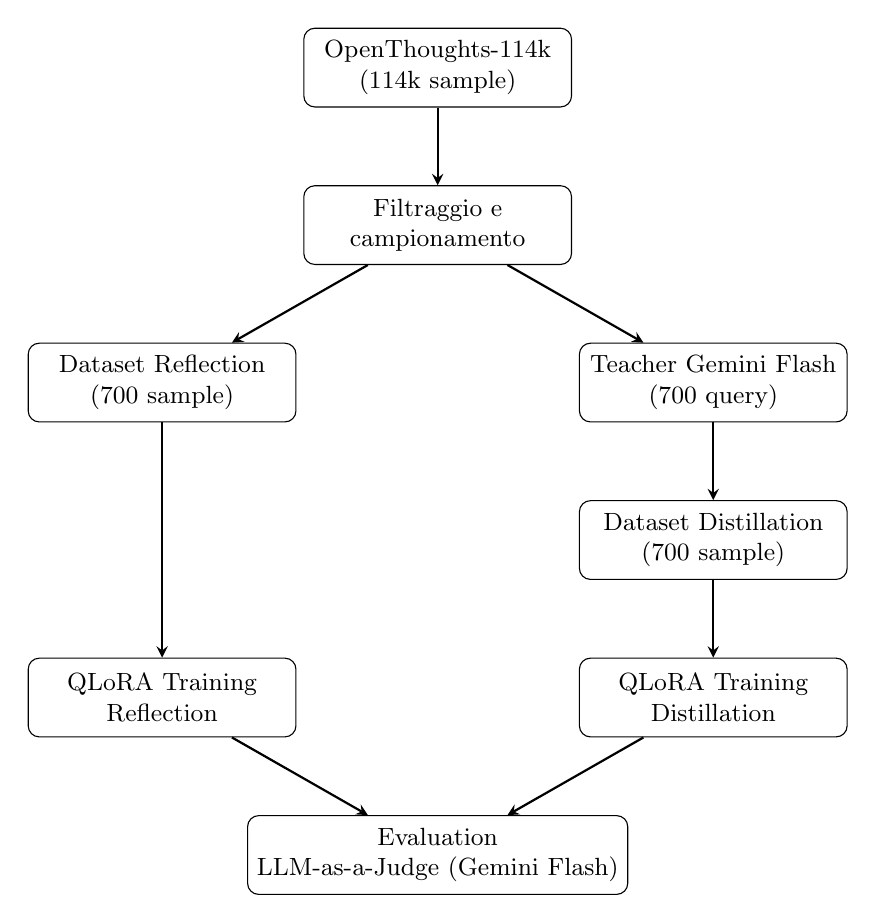
\begin{tikzpicture}[
      box/.style={rectangle, draw, rounded corners,
                  minimum width=3.4cm, minimum height=1cm,
                  align=center, font=\small},
      arrow/.style={->, thick, >=stealth}
    ]
    \node[box] (ds)   at (3.5,  0)  {OpenThoughts-114k\\(114k sample)};
    \node[box] (filt) at (3.5, -2)  {Filtraggio e\\campionamento};
    \node[box] (refl) at (0,   -4)  {Dataset Reflection\\(700 sample)};
    \node[box] (teach)at (7,   -4)  {Teacher Gemini Flash\\(700 query)};
    \node[box] (dist) at (7,   -6)  {Dataset Distillation\\(700 sample)};
    \node[box] (tr1)  at (0,   -8)  {QLoRA Training\\Reflection};
    \node[box] (tr2)  at (7,   -8)  {QLoRA Training\\Distillation};
    \node[box] (eval) at (3.5, -10) {Evaluation\\LLM-as-a-Judge (Gemini Flash)};
    \draw[arrow] (ds)    -- (filt);
    \draw[arrow] (filt)  -- (refl);
    \draw[arrow] (filt)  -- (teach);
    \draw[arrow] (teach) -- (dist);
    \draw[arrow] (refl)  -- (tr1);
    \draw[arrow] (dist)  -- (tr2);
    \draw[arrow] (tr1)   -- (eval);
    \draw[arrow] (tr2)   -- (eval);
  \end{tikzpicture}
  \caption{Schema della pipeline sperimentale. Le frecce indicano il
    flusso dei dati. I due rami di training condividono lo stesso modello
    base (Llama~3.2~1B-Instruct) e gli stessi iperparametri.}
  \label{fig:pipeline}
\end{figure}

\FloatBarrier
% ------------------------------------------------------------
\section{Preparazione del Dataset}
\label{sec:step1}
% ------------------------------------------------------------

Il dataset di partenza è \textbf{OpenThoughts-114k}
\cite{openthoughts2024}, un corpus pubblico disponibile su
Hugging Face che raccoglie oltre 114\,000 conversazioni generate da
modelli di tipo \emph{chain-of-thought}. Ogni campione è strutturato
come una conversazione a due turni: una domanda dell'utente e una
risposta dell'assistente che include un blocco di ragionamento
delimitato dai tag \texttt{<|begin\_of\_thought|>} e
\texttt{<|end\_of\_thought|>}, seguito dalla soluzione finale.

\paragraph{Filtraggio.}
Lo script \texttt{prepare\_dataset.py} applica una pipeline di
filtraggio per selezionare i campioni di qualità sufficiente.
I campioni vengono accettati solo se soddisfano tutti i vincoli
definiti nella Tabella~\ref{tab:filtri}. I campioni validi vengono
rimescolati con seed fisso (\texttt{SEED = 42}) e suddivisi in
700 campioni di training e 80 campioni di valutazione.

\begin{table}[t]
  \centering
  \caption{Criteri di filtraggio applicati ai campioni di OpenThoughts-114k.}
  \label{tab:filtri}
  \small
  \renewcommand{\arraystretch}{1.3}
  \begin{tabular}{l l p{6cm}}
    \toprule
    \textbf{Parametro} & \textbf{Valore} & \textbf{Motivazione} \\
    \midrule
    \texttt{MIN\_THINKING\_LEN} & 300 car. &
      Esclude ragionamenti troppo superficiali \\
    \texttt{MAX\_THINKING\_LEN} & 6000 car. &
      Evita sequenze che superano il contesto del modello \\
    \texttt{MIN\_ANSWER\_LEN}   & 50 car. &
      Esclude risposte degeneri o incomplete \\
    Lunghezza minima thinking   & 50 parole &
      Filtra blocchi formalmente presenti ma privi di contenuto \\
    \bottomrule
  \end{tabular}
\end{table}

\paragraph{Formato di output.}
Ciascun campione viene riformattato nel formato conversazionale
atteso dal modello: il ragionamento estratto viene racchiuso nel
tag \texttt{<thinking>...</thinking>} e concatenato alla soluzione
finale, producendo la risposta dell'assistente che lo student dovrà
apprendere a generare.

\FloatBarrier
% ------------------------------------------------------------
\section{Generazione del Dataset di Distillation}
\label{sec:step1b}
% ------------------------------------------------------------

La preparazione del dataset di distillation segue due approcci
complementari. Il primo, implementato in
\texttt{build\_distillation\_dataset.py}, genera il dataset a partire
direttamente dal dataset reflection, rimuovendo i blocchi
\texttt{<thinking>} tramite espressione regolare e conservando solo
la risposta finale. Questo produce un dataset con le stesse domande
e risposte di base, con l'unica differenza della \emph{presenza o
assenza del ragionamento esplicito}.

Il primo approccio rimuove il blocco \texttt{<thinking>} tramite
espressione regolare, conservando solo il testo successivo al tag
di chiusura:

\begin{comment}
\begin{lstlisting}[language=Python, caption={Estrazione della risposta finale dal campione reflection.}]
match = re.search(r"</thinking>\s*\n*(.*)", content, re.DOTALL)
answer_only = match.group(1).strip()
\end{lstlisting}
\end{comment}

Il secondo approccio, implementato in
\texttt{generate\_teacher\_responses.py}, interroga \textbf{Gemini
Flash} (\texttt{gemini-2.5-flash}) come modello teacher: per
ciascuna delle 700 domande viene generata una risposta diretta senza
ragionamento esplicito, configurando uno scenario di \emph{knowledge
distillation response-based} in cui lo student impara a riprodurre
le risposte di un teacher più capace. Il sistema prompt fornito al
teacher specifica esplicitamente di non utilizzare tag XML di
reasoning:

\begin{lstlisting}[language=Python, caption={System prompt inviato a Gemini Flash come teacher.}, float=tbp]
SYSTEM_PROMPT = """You are a helpful and precise assistant.
Answer the user's question clearly and correctly.
Show your reasoning when solving problems, but be concise.
Do NOT use XML tags like <thinking> in your response."""
\end{lstlisting}

Per gestire i vincoli della quota gratuita dell'API (15 richieste al
minuto), lo script implementa un meccanismo di rate limiting con sleep
inter-chiamata di circa 4.3 secondi e un sistema di checkpoint ogni
10 chiamate, consentendo la ripresa in caso di interruzione. Il tempo
complessivo per la generazione delle 700 risposte è stato di circa
50 minuti.

\FloatBarrier
% ------------------------------------------------------------
\section{Fine-Tuning con QLoRA}
\label{sec:step2}
% ------------------------------------------------------------

Entrambi i modelli sono addestrati a partire da
\textbf{Llama~3.2~1B-Instruct} \cite{meta2024llama32}, nella variante
quantizzata a 4 bit (NF4) fornita da Unsloth. La quantizzazione tramite
\texttt{bitsandbytes} riduce l'utilizzo di memoria di circa il 75\%
rispetto alla precisione float16, rendendo il training fattibile su
GPU con 16\,GB di VRAM.

\subsection{Configurazione LoRA}

L'adattamento del modello è realizzato con \textbf{Low-Rank
Adaptation} \cite{hu2021lora} tramite la libreria PEFT. I parametri
adottati sono riportati nella Tabella~\ref{tab:lora}. I moduli target
coprono sia i layer di self-attention (\texttt{q\_proj},
\texttt{k\_proj}, \texttt{v\_proj}, \texttt{o\_proj}) sia i layer
feed-forward della MLP (\texttt{gate\_proj}, \texttt{up\_proj},
\texttt{down\_proj}), massimizzando la capacità di adattamento entro
i vincoli di memoria disponibile.

\begin{table}[t]
  \centering
  \caption{Iperparametri LoRA e di training condivisi tra i due esperimenti.}
  \label{tab:lora}
  \small
  \renewcommand{\arraystretch}{1.3}
  \begin{tabular}{l l l l l l}
    \toprule
    $r$ & $\alpha$ & Dropout & LR & Epoche & Batch eff. \\
    \midrule
    16 & 32 & 0.0 & $2{\times}10^{-4}$ & 3 & 8 \\
    \bottomrule
  \end{tabular}
\end{table}

\subsection{Procedura di training}

Gli iperparametri di training sono identici per entrambi i modelli
(Tabella~\ref{tab:lora}): learning rate $2 \times 10^{-4}$ con
ottimizzatore AdamW 8-bit, 3 epoche, batch size effettivo 8
(batch~2 con gradient accumulation~4), LR scheduler cosine con
warmup ratio 0.05, lunghezza massima della sequenza 2048 token e
seed 42. Questa scelta garantisce che qualunque differenza nelle
prestazioni finali sia attribuibile esclusivamente al formato dei
dati di addestramento.

Il modello di reflection è addestrato tramite \texttt{train\_reflection.py} con \\
\texttt{UnslothTrainer}, che applica ottimizzazioni specifiche per
sequenze lunghe con reasoning tag. Il modello di distillation è
addestrato tramite \texttt{train\_distillation.py} con
\texttt{SFTTrainer} della libreria TRL, con parametri equivalenti.
Al termine del training, le sole matrici LoRA vengono salvate come
adapter separati, con dimensione su disco dell'ordine di poche decine
di MB ciascuno.

\FloatBarrier
% ------------------------------------------------------------
\section{Valutazione Comparativa}
\label{sec:step3}
% ------------------------------------------------------------

\subsection{Procedura di inferenza}

Lo script \texttt{evaluate.py} carica entrambi i modelli sequenzialmente
e genera le risposte alle stesse 20 domande del test set con parametri
di decodifica identici:

\begin{lstlisting}[language=Python, caption={Parametri di generazione usati durante la valutazione.}, float=tbp]
outputs = model.generate(
    **inputs,
    max_new_tokens = 512,
    temperature    = 0.6,
    top_p          = 0.9,
    do_sample      = True,
    pad_token_id   = tokenizer.eos_token_id,
)
\end{lstlisting}

La temperatura $T = 0.6$ bilancia diversità e coerenza delle risposte;
il nucleus sampling con $p = 0.9$ tronca la distribuzione escludendo
i token meno probabili.

\subsection{LLM-as-a-Judge}

La valutazione delle risposte è delegata a \textbf{Gemini Flash}
in qualità di giudice automatico, secondo il paradigma
\emph{LLM-as-a-Judge} \cite{zheng2023judging}. Ad ogni coppia
di risposte viene sottoposto un prompt strutturato che richiede
al giudice di assegnare punteggi su tre dimensioni:

\begin{enumerate}
  \item \textbf{Correctness} (1--5): correttezza della risposta finale
  \item \textbf{Reasoning Quality} (1--5): qualità e coerenza del
    ragionamento mostrato
  \item \textbf{Clarity} (1--5): chiarezza e struttura espositiva
\end{enumerate}

e di indicare il vincitore complessivo tra i due modelli (A, B, o
parità). Il prompt sottoposto al giudice segue il template:

\begin{lstlisting}[language=Python, caption={Template del prompt per il giudice LLM.}, float=tbp]
JUDGE_PROMPT = """You are an expert evaluator comparing two AI
responses to a reasoning question.

Question: {question}
Model A (Distillation) response: {response_a}
Model B (Reflection)  response: {response_b}

Evaluate both on: CORRECTNESS, REASONING_QUALITY, CLARITY (1-5).
Then decide: which model is BETTER overall? (A, B, or TIE)

Respond ONLY in this JSON format:
{
  "model_a": {"correctness": 0, "reasoning_quality": 0, "clarity": 0},
  "model_b": {"correctness": 0, "reasoning_quality": 0, "clarity": 0},
  "winner": "A|B|TIE",
  "reasoning": "brief explanation"
}"""
\end{lstlisting}

Il giudice restituisce i risultati in formato JSON strutturato,
che viene parsato e salvato in \texttt{evaluation\_results.csv}.
Per contenere il numero di token inviati al giudice, le risposte
vengono troncate a 1000 caratteri. Il training è stato eseguito
interamente su \textbf{Google Colab} con GPU \textbf{NVIDIA Tesla T4}
(16\,GB VRAM) tramite la libreria Unsloth, che ottimizza le operazioni
di attenzione e il gradient checkpointing per sequenze lunghe.
